\documentclass{scrartcl}
 
\usepackage[utf8]{inputenc}
\usepackage[T1]{fontenc}
\usepackage{lmodern}
\usepackage[pdftex]{graphicx}
\usepackage[ngerman]{babel}
\usepackage{amsmath}
\usepackage{amssymb}
\usepackage{tabularx}
\usepackage{multirow}
\usepackage{amsfonts}
\usepackage{tabto}
\usepackage{mathtools}
\TabPositions{0.1in, 0.4in, 0.6in, 0.8in, 1.0in, 1.2in, 3.4in}

\begin{document}
\begin{Large}
Aufgabe 12.1\\[0.0cm]
\end{Large}

\textbf{Zu zeigen: }Ein gleichschenkliges Dreieick (im $\mathbb{R}^2)$, dessen Basis in der $x_1$-Achse
liegt, wird durch eine komponentenweise positiv-affine Transformation in ein gleichschenkliges Dreieck,
dessen Basis auf einer Parallelen zur $x_1$-Achse liegt, überführt. \\

\textbf{Beweis: }Wir haben ein gleichschenkliges Dreieck gegeben, dessen Basis in der $x_1$-Achse liegt.
Daher wissen wir folgendes über die drei Eckpunkte $A, B$ und $C$: \\

\begin{itemize}
\item{$A = (a_1, a_2) = (a_1, 0)$}
\item{$B = (b_1, b_2) = (a_1 + c, 0$)}
\item{$C = (c_1, c_2) = (a_1 + \frac{c}{2}, c_2$)}
\end{itemize}

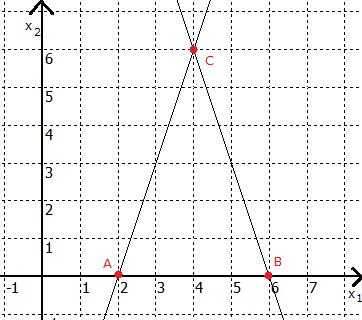
\includegraphics{triangle.png} \\

Sei $\alpha x + \beta$ eine komponentenweise positiv-affine Transformation von $x \in \mathbb{R}^2$, d.h.
$\alpha > 0$ und $\beta \in \mathbb{R}^2$. Wir wenden diese Transformation auf $A, B$ und $C$ an: \\

\begin{itemize}
\item{$A' = \alpha A + \beta = (\alpha_1 a_1 + \beta_1, 0 + \beta_2)$}
\item{$B' = \alpha B + \beta = (\alpha_1 \cdot (a_1 + c) + \beta_1, 0 + \beta_2$)}
\item{$C' = \alpha C + \beta = (\alpha_1 \cdot (a_1 + \frac{c}{2}) + \beta_1, \alpha_2 c_2 + \beta_2$)}
\end{itemize}

Wir stellen fest: \\

\begin{itemize}
\item{$A'$ und $B'$ haben beide den $x_2$-Wert $\beta_2 \Rightarrow A'$ und $B'$ liegen auf der Parallele
zur $x_1$-Achse durch $(0, \beta_2)$. $\overline{A'B'}$ ist die Basis des gleichschenkligen Dreiecks.}
\item{Die Distanz zwischen $A'$ und $B'$ beträgt $\alpha_1 \cdot (a_1 + c) + \beta_1 - (\alpha_1 a_1 +
\beta_1) = \alpha_1 \cdot c$. Die Differenz der $x_1$-Werte von $A$ und $C$ beträgt $\alpha_1 \cdot (a_1 +
\frac{c}{2}) + \beta_1 - (\alpha_1 a_1 + \beta_1) = \alpha_1 \cdot \frac{c}{2}$. Das ist genau
die Hälfte der Differenz der $x_1$-Werte von $A'$ und $B' \Rightarrow C'$ liegt auf der Mittelsenkrechten
zu $\overline{A'B'}$.}
\end{itemize}

Da $A'B'$ parallel zur $x_1$-Achse ist und $C'$ auf der Mittelsenkrechten zu $A'B'$ liegt, ist $A'B'C'$
ein gleichschenkliges Dreieck, dessen Basis auf einer Parallelen zur $x_1$-Achse liegt. \clearpage

\begin{Large}
Aufgabe 12.3\\[0.0cm]
\end{Large}

a) \\

Wir zeigen, dass $(\frac{3}{4}, \frac{3}{4})$ die Nash-Lösung für das Spiel $(S, d)$ ist. \\

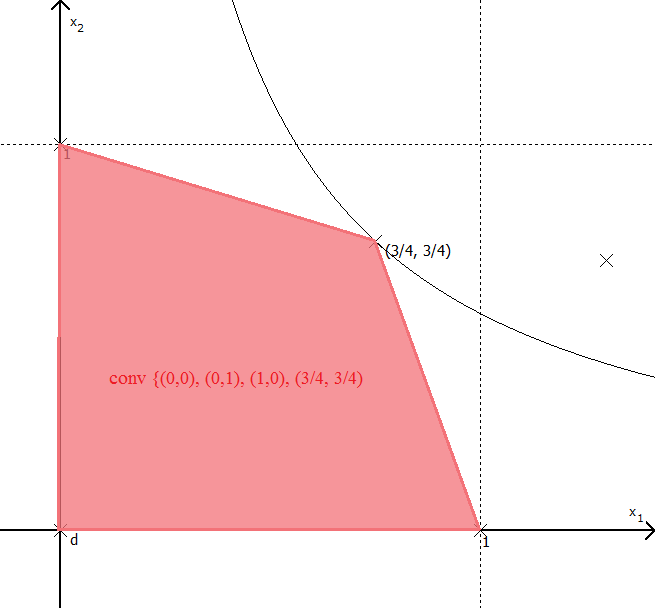
\includegraphics[width=12cm]{3a.png} \\

Dazu zeigen wir einfach, dass $x =(\frac{3}{4}, \frac{3}{4})$ die Alternative $x \in S$ ist, welche die Fläche
des Rechtecks mit unterer linker Ecke $d$ und oberer rechter Ecke $x$ maximiert. \\

In der Abbildung ist neben $S$ noch ein Teil der Funktion $x_2(x_1) = (\frac{3}{4})^2 \cdot \frac{1}{x_1}$
eingezeichnet, sprich dies sind genau die Punkte $(x_1, x_2)$ mit $x_1 \cdot x_2 = (\frac{3}{4})^2$. Für die
Punkte auf dieser Kurve ist der Flächeninhalt des Rechtecks mit unterer linker Ecke $d$ und oberer Rechter
Ecke $x = (x_1, x_2)$ genau $(\frac{3}{4})^2$. \\

Für $x$ oberhalb dieser Kurve ist der Flächeninhalt größer, für $x$ unterhalb kleiner. Da die Kurve genau durch
$(\frac{3}{4}, \frac{3}{4})$ verläuft und $S$ mit Ausnahme von $(\frac{3}{4}, \frac{3}{4})$ komplett unterhalb der
Kurve liegt, ist $(\frac{3}{4}, \frac{3}{4})$ die Nash-Lösung für dieses Spiel.


\end{document}